\documentclass[12pt, a4paper]{article}

\usepackage{listings}
\usepackage{color}
\usepackage{enumitem}
\usepackage{amsthm}
\usepackage{amssymb}
\usepackage{listings}
\usepackage{setspace}
\usepackage{graphicx}
\graphicspath{ {./figures/} }


\title{Introduction to Neurobiology}
\author{William Darko}
\date{Summer 2021}

\pagenumbering{arabic}

\begin{document}

\maketitle
\newpage

\tableofcontents

\newpage

\section{About this course}
\paragraph*{}
Objective of the course is to learn how the nervous system produces behaviour,
how we use our brains in our day to day lives, and how neuroscience can help explain
the problems afflicting people today. There'll be focus on functional human neuroanatomy,
and neuronal communication, to help understand how we perceive the world, do body movements,
and interact with others.

\newpage

\section{Resources}

\begin{itemize}
    \item \textbf{Coursera: Understanding the Brain: The Neurobiology of Everyday Life}
    taught by professor of Neurobiology Peggy Mason, at the University of Chicago (https://www.coursera.org/learn/neurobiology)
\end{itemize}

\newpage

\section{Introduction}
\begin{itemize}
    \item \textbf{The Diving Bell and the Butterfly}: 
    Jean-Dominique Bauby, locked-in syndorme.
\end{itemize}

\section{The Nervous System}
\subsection{The Four Functions}
The locked-in syndrome tells of the four basic functions of the brain/central nervous system.
\begin{enumerate}
    \item \textbf{Voluntary Movement:} Every thing we do that is driven by the brain,
    both deliberate actions, such jumping, speaking, raising your hand, etc, and not so deliberate
    actions like wincing in reaction to stepping on a lego piece.
    \item \textbf{Perception:} Perception is distinct from sensation; its what we conciously
    appreciate about sensation. Its what we're capable of being aware of such as vision, hearing,
    smell, taste, balance, position, lung pressure, etc.
    \item \textbf{Homeostasis:} Used to keep body within its physiological limits.
    For example, making sure the body has enough oxygen, the right blood pressure, right body temperature.
    Also, homeostasis accounts for life cycle events like a mother giving birth, and the conditions 
    needed for the child to be healthy. Altogether, a process of maintaining healthy internal conditions.
    \item \textbf{Abstract functions:} Higher functions of the central nervous system like
    thinking, language, motivation, feeling emotion, etc. Also, plays a huge role in how we interact with other humans.
\end{enumerate}

\subsection{Central Anatomy}
Mapping of the four functions to regions of the brain.
\begin{enumerate}
    \item Motor neurons which exist in the brain stem, or the spinal cord are responsible
    for \textbf{voluntary movement}. There are less than 100,000 motor neurons, out of about 200 billion
    in the entire nervous system. Motor neurons in the brain system are responsible of movement of the mouth, face,
    hence speech, facial expressions, swallowing, etc.
    Motor neurons in the spinal cord are responsible for bodily movements like movement of the arms,
    legs, etc.
    \item \textbf{Perception} is entirely in the \textbf{Forebrain}; more specifically,  it depends entirely on the \textbf{Cerebral Cortex}.
    Perception is one of the higher brain functions; if the information carried by neurons does not 
    make it to to the Cerebral Cortex, then there's no perception; there's no concious appreciation/awareness
    of sensation.
    \item \textbf{Homeostasis} depends on the \textbf{Forebrain, brain stem, and spinal cord}.
    The forbrain's contribution to homeostasis is hormonal. The brain stem has a varied contribution; its responsible for
    the automatic changes we're not able to control, the autonomic (involuntary) functions of our nervous system. The spinal cord's
    contribution is similar to that of the brain stem.
    
    The brain stem, and spinal cord serve as pathways for information, both incoming, and outgoing. 

    \item \textbf{Abstract functions} are entirely in the forebrain, and function independent of the brain stem, and spinal cord.
    The forebrain is the "seat of conciousness"; all perception, and abstract conginitve functions like memory, depend on the forebrain;
    more specifically,the cerebral cortex.
\end{enumerate}

{
    \centering
    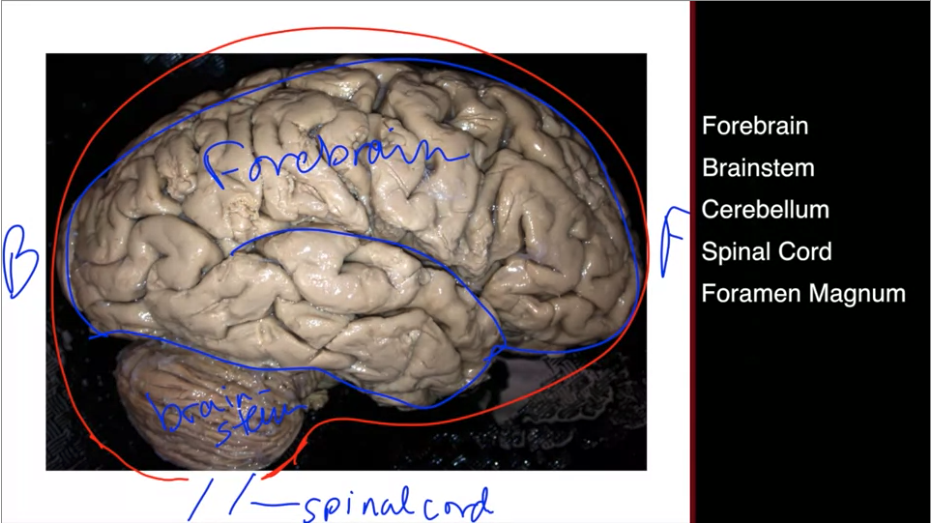
\includegraphics[width=8cm]{BrainImg_FromSide_SidesAnnotated.png}
    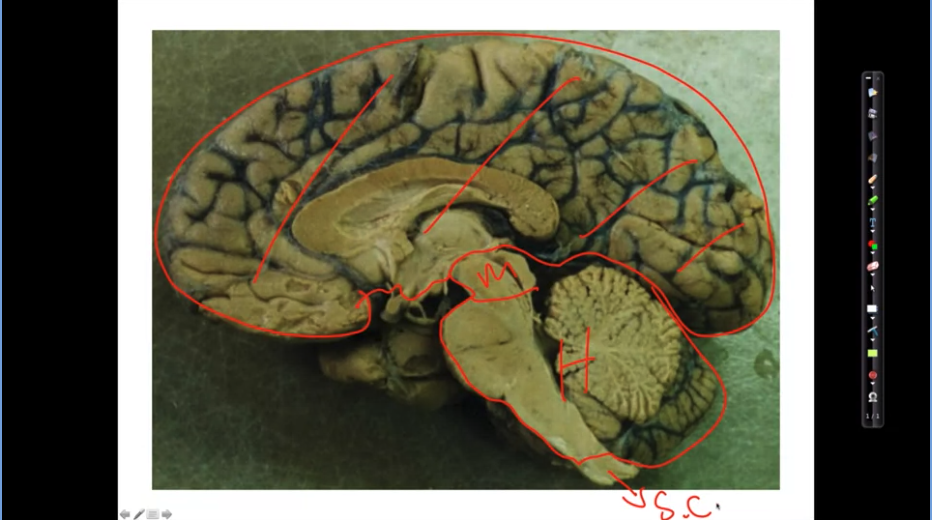
\includegraphics[width=8cm]{BrainImg_CutFromSide_MidHindBrainStem.png}

}
\newpage

\section{Neurons}

\end{document}